\chapter{Desenvolvimento}

A seção de desenvolvimento de um relatório técnico é a parte central do documento, onde são detalhadas as atividades a serem realizadas e os métodos inicialmente planejados para serem empregados. Esta seção é dividida em subseções que podem variar de acordo com a natureza do projeto. 
Nesta parte do documento, é esperado que o autor faça uso dos conhecimentos de Engenharia de Software e áreas afins para estabelecer as bases do projeto a ser elaborado. Informações como regras de negócios, domínio da aplicação, metodologias e métodos de desenvolvimento, requisitos e funcionalidades, persistência de dados são apenas algumas das informações que poderão ser necessárias a depender do projeto proposto.  Em geral, algumas seções a serem incluídas são: 

\begin{itemize}
    \item Metodologia: Descrição detalhada das técnicas e processos que devem ser utilizados no desenvolvimento do projeto, incluindo ferramentas, linguagens de programação, frameworks e metodologias de desenvolvimento de software. Indicar quais são os principais fundamentos (algoritmos, paradigmas, teorias) a serem empregados. Cada fundamento utilizado deve ser justificado. Indicar também quais são as principais tecnologias (ambientes de desenvolvimento, linguagens de programação, plataformas de hardware) a serem empregadas. Cada tecnologia utilizada deve ser justificada. 

    \item Implementação: Detalhamento da construção do sistema ou aplicação, abordando aspectos como arquitetura de software, módulos desenvolvidos, funcionalidades implementadas e interfaces de usuário.

    \item Testes: Apresentação das estratégias de teste que serão adotadas, incluindo testes unitários, de integração, de sistema e de aceitação.

    \item Resultados esperados: Exposição dos resultados a serem alcançados com o desenvolvimento do projeto, podendo incluir métricas de desempenho, feedback dos usuários, impacto nos processos ou práticas existentes e contribuições para a área de conhecimento.
\end{itemize}


Para organizar todas estas informações, o autor precisará fazer uso de seções e subseções. As explicações sobre como proceder com a formatação destes recursos são apresentadas a seguir.

\section{Funcionalidades}

Descreva nesta seção as funcionalidades que a ferramenta ou produto de software terá após seu desenvolvimento. Cada funcionalidade deve ser explicada de forma clara e completa, de modo que qualquer leitor possa entender exatamente o que o software faz e como ele atende às necessidades identificadas na seção de descrição da regra de negócio.
Sugere-se que as funcionalidades da ferramenta ou produto de software sejam apresentadas de forma organizada, agrupando-as por módulos e categorias, se aplicável. Por exemplo, se o software tem um módulo de administração e um módulo de usuário, agrupe as funcionalidades de acordo. A seguir é apresentada uma sugestão de itens a serem abordados para cada funcionalidade, ficando claro que é só uma sugestão e que o orientador deverá ser consultado a respeito.

\subsection{Funcionalidade 1}
\begin{itemize}
    \item \textbf{Nome da Funcionalidade}: Dê um nome claro e descritivo.
    \item \textbf{Objetivo}: Explique o propósito da funcionalidade e o problema específico que ela resolve.
    \item \textbf{Descrição}: Detalhe como a funcionalidade funciona, incluindo fluxos de trabalho, interações com o usuário e exemplos práticos de uso.
    \item \textbf{Requisitos}: Liste os requisitos necessários para a funcionalidade, como dados de entrada, pré-condições e pós-condições.
    \item \textbf{Interfaces}: Descreva a interface do usuário relacionada à funcionalidade, se aplicável, incluindo capturas de tela, wireframes ou protótipos.
    \item \textbf{Exemplo de Uso}: Forneça um exemplo concreto de como a funcionalidade é utilizada na prática, idealmente com um cenário realista ou um caso de uso.
\end{itemize}

\section{Persistência de dados}

Na Seção de "Persistência de Dados", os estudantes devem explicar como os dados são armazenados, gerenciados e recuperados pelo software. Isso inclui a descrição da estrutura do banco de dados, o modelo de dados adotado, as tecnologias utilizadas, e exemplos de consultas e operações realizadas sobre os dados. 
Sugere-se que sejam apresentadas todas as estruturas e modelos que são necessários para compreensão da persistência dos dados na ferramenta ou produto de software a ser desenvolvido, como Diagramas ER, esquemas de tabelas e fluxogramas. Além disso, a inclusão de detalhes técnicos específicos, como tipos de dados, restrições de integridade e exemplos de consultas SQL é importante para melhor compreensão. 


\section{Tecnologias Utilizadas}
% SEÇÃO ORIBRIGATÓRIA PARA TCC 2 E OPCIONAL PARA O TCC 1 

Nesta seção, os estudantes devem listar e descrever as principais tecnologias utilizadas no desenvolvimento do software. Isso inclui linguagens de programação, frameworks, bibliotecas, ferramentas de desenvolvimento, plataformas e serviços externos. A explicação deve detalhar o papel de cada tecnologia e justificar sua escolha.
Se possível, detalhe as versões específicas das tecnologias usadas e explique qualquer configuração ou customização realizada, e explique como cada tecnologia suportou a implementação das funcionalidades descritas anteriormente. 

\section{Avaliação/Testes}
% SEÇÃO ORIBRIGATÓRIA PARA TCC 2 E OPCIONAL PARA O TCC 1 

Esta seção é dedicada a descrição do processo de avaliação e testes realizados no software. Isso inclui os tipos de testes aplicados, as ferramentas utilizadas, os resultados obtidos e como esses resultados foram usados para melhorar o sistema.

\section{Cronograma}
% SEÇÃO ORIBRIGATÓRIA PARA TCC 1. 
% DEVE SER REMOVIDA PARA O TCC 2

A subseção Cronograma de um relatório técnico é fundamental para organizar e planejar as etapas do projeto ao longo do tempo. Geralmente apresentado em forma de tabela ou gráfico de Gantt, o cronograma lista as atividades, suas datas de início e término previstas, e a duração. Isso ajuda a visualizar a sequência das tarefas, identificar períodos críticos e monitorar o andamento do projeto. É uma ferramenta essencial para garantir que o trabalho seja concluído dentro do prazo estipulado.
Devem estar detalhadas, de forma lógica, linear e cronológica, todas as etapas do projeto que esclareçam como o produto será gerado. 

\section{Como utilizar figuras}

São ilustrações: figuras, quadros, gráficos, fotografias, retratos, desenhos, gravuras, imagens, fluxogramas, organogramas, esquemas, mapas, plantas e diferenciam-se das tabelas. As ilustrações devem ser inseridas o mais próximo possível do texto a que se refere.
Qualquer que seja o tipo de ilustração, sua identificação aparece na parte inferior, precedida da palavra designativa, seguida de seu número de ordem de ocorrência no texto, em algarismos arábicos, do respectivo título e/ou legenda. A fonte deve ser tamanho 10 e em negrito. Após a legenda, deve-se citar a fonte de onde foi retirada a ilustração, precedida da palavra “Fonte” (Autor, data), bem como, deve-se referenciá-la, de forma completa, na seção Referências.

Na Figura~\ref{fig:dummy} \'e apresentado um exemplo de gr\'afico flutuante. Esta figura aparece automaticamente na lista de figuras. Para uso avan\c{c}ado de gr\'aficos no \LaTeX, recomenda-se a consulta de literatura especializada~\cite{Goossens2007}.


\begin{figure}[!htb]
	\centering
	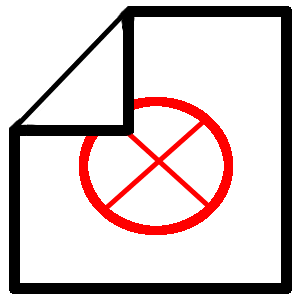
\includegraphics[width=0.2\textwidth]{Imagens/dummy.png} % <- formatos PNG, JPG e PDF
	\caption[Exemplo de uma figura]{Exemplo de uma figura onde aparece uma imagem sem nenhum significado especial.}
	\fonte{\cite{abnTeX2009}}
	\label{fig:dummy}
\end{figure}


\section{Como utilizar tabelas}

Uma tabela deve apresentar dados numéricos de modo resumido e é utilizada principalmente para a apresentação de comparações. Deve-se seguir tal padrão em todo o trabalho, constando também na lista de tabelas, separada da lista de ilustrações. Os quadros não devem ser chamados de tabelas, uma vez que se diferenciam destas por apresentarem as laterais fechadas e o conteúdo não numérico\footnote{Para as regras gerais de apresentação de tabelas, ver página 61 das Normas para Elaboração de Trabalhos Acadêmicos da UTFPR, dispon\'ivel em: http://www.utfpr.edu.br/documentos/normas\_trabalhos\_utfpr.pdf}.

Tamb\'em \'e apresentado o exemplo da tabela~\ref{tab:correlacao}, que aparece automaticamente na lista de tabelas. Informa\c{c}\~oes sobre a constru\c{c}\~ao de tabelas no \LaTeX\ podem ser encontradas na literatura especializada~\cite{Lamport1986,Buerger1989,Kopka2003,Mittelbach2004}.

\begin{table}[!htb]
	\centering
	\caption[Exemplo de uma tabela]{Exemplo de uma tabela mostrando a correla\c{c}\~ao entre x e y.}
	\label{tab:correlacao}
	\begin{tabular}{cc}
		\hline 
		x & y \\
		\hline
		1 & 2 \\
		3 & 4 \\
		5 & 6 \\
		7 & 8 \\
		\hline 
	\end{tabular}
	\fonte{Autoria pr\'opria.}
\end{table}

\section{Como utilizar equações}

A transformada de Laplace \'e dada na equa\c{c}\~ao~(\ref{eq:laplace}), enquanto a equa\c{c}\~ao~(\ref{eq:dft}) apresenta a formula\c{c}\~ao da transformada discreta de Fourier bidimensional\footnote{Deve-se reparar na formata\c{c}\~ao esteticamente perfeita destas equa\c{c}\~oes!}.

\begin{equation}
X(s) = \int\limits_{t = -\infty}^{\infty} x(t) \, \text{e}^{-st} \, dt
\label{eq:laplace}
\end{equation}

\begin{equation}
F(u, v) = \sum_{m = 0}^{M - 1} \sum_{n = 0}^{N - 1} f(m, n) \exp \left[ -j 2 \pi \left( \frac{u m}{M} + \frac{v n}{N} \right) \right]
\label{eq:dft}
\end{equation}

\section{Como utilizar siglas e símbolos}

O pacote \textsc{abn}\TeX\ permite ainda a defini\c{c}\~ao de siglas e s\'imbolos com indexa\c{c}\~ao autom\'atica atrav\'es dos comandos {\ttfamily \textbackslash sigla\{\}\{\}} e {\ttfamily \textbackslash simbolo\{\}\{\}}. Por exemplo, o significado das siglas\sigla{CPGEI}{Programa de P\'os-gradua\c{c}\~ao em Engenharia El\'etrica e Inform\'atica Industrial},\sigla{DAELN}{Departamento Acad\^emico de Eletr\^onica} e\sigla{UTFPR}{Universidade Tecnol\'ogica Federal do Paran\'a} aparecem automaticamente na lista de siglas, bem como o significado dos s\'imbolos\simbolo{$\lambda$}{comprimento de onda},\simbolo{$v$}{velocidade} e\simbolo{$f$}{frequ\^encia} aparecem automaticamente na lista de s\'imbolos. Mais detalhes sobre o uso destes e outros comandos do \textsc{abn}\TeX\ s\~ao encontrados na sua documenta\c{c}\~ao espec\'ifica~\cite{abnTeX2009}.


\section{Seção Secundária}

\subsection{Seção Terciária}

Seção terciária \cite{Lamport1986, Kopka2003}

\subsubsection[Seção quaternária]{\underline{Seção quaternária}}

Seção quaternária.